\documentclass[a4paper,english,12pt]{article}
\usepackage{%
	amsfonts,%
	amsmath,%	
	amssymb,%
	amsthm,%
	algorithm,%
	babel,%
	bbm,%
	etex,%
	%biblatex,%
	caption,%
	centernot,%
	color,%
	dsfont,%
	enumerate,%
	epsfig,%
	epstopdf,%
	geometry,%
	graphicx,%
	hyperref,%
	latexsym,%
	mathtools,%
	multicol,%
	pgf,%
	pgfplots,%
	pgfplotstable,%
	pgfpages,%
	proof,%
	psfrag,%
	subfigure,%	
	tikz,%
	ulem,%
	url%
}	
\usepackage[noend]{algpseudocode}
\usepackage[mathscr]{eucal}
\usepgflibrary{shapes}
\usetikzlibrary{%
  	arrows,%
	backgrounds,%
	chains,%
	decorations.pathmorphing,% /pgf/decoration/random steps | erste Graphik
	decorations.text,%
	matrix,%
  	positioning,% wg. " of "
  	fit,%
	patterns,%
  	petri,%
	plotmarks,%
  	scopes,%
	shadows,%
  	shapes.misc,% wg. rounded rectangle
  	shapes.arrows,%
	shapes.callouts,%
  	shapes%
}

\theoremstyle{plain}
\newtheorem{thm}{Theorem}[section]
\newtheorem{lem}[thm]{Lemma}
\newtheorem{prop}[thm]{Proposition}
\newtheorem{cor}[thm]{Corollary}

\theoremstyle{definition}
\newtheorem{defn}[thm]{Definition}
\newtheorem{conj}[thm]{Conjecture}
\newtheorem{exmp}[thm]{Example}
\newtheorem{assum}[thm]{Assumptions}
\newtheorem{axiom}[thm]{Axiom}

\theoremstyle{remark}
\newtheorem{rem}{Remark}
\newtheorem{note}{Note}
\newtheorem{fact}{Fact}

\newcommand{\norm}[1]{\left\lVert#1\right\rVert}
\newcommand{\indep}{\!\perp\!\!\!\perp}
\DeclarePairedDelimiter\abs{\lvert}{\rvert}%
\newcommand\numberthis{\addtocounter{equation}{1}\tag{\theequation}}
\newcommand{\tr}{\operatorname{tr}}
\newcommand{\R}{\mathbb{R}}
\newcommand{\N}{\mathbb{N}}
\newcommand{\E}{\mathbb{E}}
\newcommand{\Z}{\mathbb{Z}}
\newcommand{\B}{\mathscr{B}}
\newcommand{\C}{\mathcal{C}}
\newcommand{\T}{\mathscr{T}}
\newcommand{\F}{\mathcal{F}}
\newcommand{\G}{\mathcal{G}}
%\newcommand{\ba}{\begin{align*}}
%\newcommand{\ea}{\end{align*}}
\DeclareMathOperator*{\argmax}{arg\,max}
\renewcommand{\qedsymbol}{$\blacksquare$}
\makeatletter
\def\BState{\State\hskip-\ALG@thistlm}
\makeatother

\makeatletter
\def\th@plain{%
  \thm@notefont{}% same as heading font
  \itshape % body font
}
\def\th@definition{%
  \thm@notefont{}% same as heading font
  \normalfont % body font
}
\makeatother
\date{}
\usepackage{algorithm,algpseudocode}
\newcommand{\uphi}{\underline{\phi}}
\newcommand{\udel}{\underline{\delta}}
\newcommand{\te}{\textrm}
\title{Lecture 15: Chernoff bounds and Sequential detection}
\date{01 March 2016}
\begin{document}
\author{}
\maketitle
\section{Chernoff Bounds}
\subsection{Bayesian Hypothesis Test}
A test using log-likelihood ratio statistic has the form,
\begin{equation}
T(Y)=\log{L(Y)}\gtreqqless \tau.
\end{equation}
\textbf{Bound-1:}
The probability of error $P_e$ is bounded as,
\begin{equation}
P_e\leq(\pi_0+\pi_1e^\tau)e^{\mu_{T,0}(s_0)-s_0\tau},
\end{equation}
where $\mu_{T,0}(s)=\log\mathbb{E}_0[e^{sT(y)}]$, and $\mu^{'}_{T,0}(s_0)=\tau$.\\
\textbf{Bound-2:}
$\forall\ s\in[0,1]$,
\begin{equation}
P_e\leq \max(\pi_0,\pi_1e^\tau)e^{\mu_{T,0}(s)-s\tau}.
\end{equation}
\textbf{Derivation of the above bound:} Consider,
\begin{align} 
P_e &=\pi_0 P_0(\Gamma_1) + \pi_1 P_1(\Gamma_0),\nonumber\\
&=\pi_0\int_{\Gamma_1}dP_0(y) + \pi_1\int_{\Gamma_0}dP_1(y).
\end{align}
Now we have,
\begin{align} 
\Gamma_1&=\{ y:T(y)>\tau\} = \{ y:\log{L(y)}>\tau\},\nonumber\\
&= \{ y:\exp\left( s\log{L(y)}\right) > \exp( s\tau)\},\ \forall\ s\geq0.
\end{align}
Therefore we have,
\begin{align}
\int_{\Gamma_1}dP_0(y)&\leq \int_{\Gamma_1}\exp( s\log{L(y)}-s\tau)~dP_0(y),\\
&=e^{-s\tau}\int_{\Gamma_1}L(y)^s \:dP_0(y).
\end{align}
Similarly for $ \int_{\Gamma_0}dP_1(y)$, we have,
\begin{equation}
\int_{\Gamma_0}dP_1(y)\leq e^{(1-s)\tau}\int_{\Gamma_0}L(y)^s \:dP_0(y).
\end{equation}
Therefore, we get,
\begin{align}
P_e&\leq\pi_0e^{-s\tau}\int_{\Gamma_1}L(y)^s \:dP_0(y)  +\pi_1e^{(1-s)\tau}\int_{\Gamma_0}L(y)^s \:dP_0(y),\\\nonumber
&\leq \max(\pi_0,\pi_1e^\tau)e^{-s\tau}\underbrace{\left[\int_{\Gamma_1}L(y)^s \:dP_0(y)+\int_{\Gamma_0}L(y)^s \:dP_0(y)\right]}_{\mathbb{E}_0[\exp(s\log{L(y)})]},
\end{align}
here $\mathbb{E}_0\left[\exp(s\log{L(y)})\right] =\exp\left(\mu_{T,0}(s)\right)$.
Therefore,
\begin{equation}
P_e \leq \max\left(\pi_0,\pi_1e^\tau \right) \exp\left(\mu_{T,0}(s)-s\tau\right).
\end{equation}
In particular, consider the minimum probability of error detector,
\begin{equation} \tau =\log\left(\frac{\pi_0}{\pi_1} \right) 
\end{equation}
For this detector, bound-2 gives,
$\forall \:s\in\left[ 0,1\right]$, 
\begin{equation}P_e \leq \pi_0^{1-s}\pi_1^{s}\exp\left(\mu_{T,0}\left( s\right) \right).
\end{equation}
\subsection{Chernoff bound for Quadratic Detector:}
\begin{align*}
&H_0:~\underline{Y}=\underline{N}\\
{versus}\\ 
&H_1:~\underline{Y}=\underline{S}+\underline{N}
\end{align*}
where $ \underline{N} \sim \mathcal{N}(0,\sigma^2 I)$, $ \underline{S} \sim \mathcal{N}(0,\Sigma_s)$ and $ \underline{S}$ is independent of $ \underline{N}$.
\paragraph{Optimal detector:}
Let,
\begin{equation}
\Sigma_s=\sum_{k=1}^{n}\lambda_k\, \underline{v_k}\:\underline{v_k^T},
\end{equation}
where $\underline{v_k}$ is an orthonormal set.
\paragraph{Test Statistic:} 
$\underline{y}^TQ\underline{y}=\sum_{k=1}^{n}\overline{y}_k^2$,
 $\te{where}\ Q=(\Sigma_0^{-1}-\Sigma_1^{-1})$, and,
\begin{equation}
\overline{y}_k=\sqrt{ \frac{\lambda_k}{\sigma^2(\sigma^2+\lambda_k)}} \:\underline{v}_k^T\underline{y}.
\end{equation}
$\{\overline{y}_k\}_{k=1}^n$ are independent and zero mean Gaussian random variables with variances $\{\sigma_{j,k}\}_{k=1}^n$,
\begin{equation}\{\sigma_{j,k}\}_{k=1}^n=\begin{cases}
\frac{\lambda_k}{\sigma^2+\lambda_k} & \text{if}\ j=0 ,\\
\frac{\lambda_k}{\sigma^2}& \text{if}\ j=1.
\end{cases}
\end{equation}
Therefore,
\begin{eqnarray}
L(\underline{y})&=&\prod_{k=1}^{n}\frac{\frac{1}{\sigma_{1k}\sqrt{2\pi}}\exp\left(-\frac{\overline{y}_k^2}{2\sigma_{1k}^2} \right) }{\frac{1}{\sigma_{0k}\sqrt{2\pi}}\exp\left(-\frac{\overline{y}_k^2}{2\sigma_{0k}^2} \right)},\nonumber\\
&=&\prod_{k=1}^{n}\left(\frac{\sigma_{0k}}{\sigma_{1k}} \right) \exp\left(-\frac{\overline{y}_k^2}{2}\left(\frac{1}{\sigma_{1k}^2}-\frac{1}{\sigma_{0k}^2} \right)  \right),\nonumber\\
&=&\prod_{k=1}^{n}\left(\frac{\sigma_{0k}}{\sigma_{1k}} \right) \exp\left(\frac{\overline{y}_k^2}{2}\right).
\end{eqnarray}
with $T=\log{L}$,
\begin{eqnarray}
\mu_{T,0}(s)&=&\log{\mathbb{E}_0\left[\exp(sL)\right]},\nonumber\\
&=&\log{\mathbb{E}_0\left[\prod_{k=1}^{n}\left(\frac{\sigma_{0k}}{\sigma_{1k}} \right)^{s} \exp\left(\frac{s\overline{y}_k^2}{2}\right)\right]},\nonumber\\
&=&\sum_{k=1}^{n}s\log\left(\frac{\sigma_{0k}}{\sigma_{1k}} \right) + \sum_{k=1}^{n}\log{\mathbb{E}_0\left[\exp\left( \dfrac{s\overline{y}_k^2}{2}\right) \right]}.
\end{eqnarray}
here, $ Y_k^2 \sim \Gamma\left(\frac{1}{2},\frac{1}{2\sigma_{0k}^2} \right) $, under $ H_0 $.
\begin{equation}
\mathbb{E}_0\left[\exp\left( \dfrac{s\overline{y}_k^2}{2}\right) \right]=\begin{cases}
\left( 1-s\sigma_{0k}^2\right)^{-\frac{1}{2}} & \text{if $s<\frac{1}{\sigma_{0k}^2}$} ,\\
\infty& \text{if $s\geq\frac{1}{\sigma_{0k}^2}$}.
\end{cases}
\end{equation}
So, the probability of error is given by,
\begin{equation}
P_e \leq \pi_0^{1-s}\pi_1^{s}\exp\left\lbrace\sum_{k=1}^{n}s\log\left(\frac{\sigma_{0k}}{\sigma_{1k}} \right) + \sum_{k=1}^{n}\left( 1-s\sigma_{0k}^2\right)^{-\frac{1}{2}} \right\rbrace \;\forall \:s\in\left[ 0,1\right].
\end{equation}
Minimizing RHS over $\:s\in[0,1], i.e., \frac{d}{ds}[RHS]=0$, we get,
\begin{equation}
\sum_{k=1}^{n}\frac{\lambda_k}{2\left(\sigma^{2} +(1-s_0)\lambda_k\right)}=\sum_{k=1}^{n}\log\left(1+\frac{\lambda_k}{\sigma^2} \right)+\log\left(\frac{\pi_1}{\pi_0} \right).
\end{equation}
\section{Sequential Detection:}
All the detectors discussed are of fixed size, i.e., number of samples is fixed and we optimized the performance of the detectors. Now we fix the desired performance and vary the number of samples to achieve the performance. The detector which uses random number of samples based on the observation sequence is called ``sequential detector". The observations $\{Y_k,~k=1,2,\dots\}$ are i.i.d distributed according to 
\begin{align*}
H_0 &: Y_k\sim P_0,~k=1,2,\dots\\
versus\\
H_1 &: Y_k\sim {P}_1,~k=1,2,\dots
\end{align*}
where $P_0\neq P_1$ are distributions on $\mathbb{R}$.
\begin{defn}
A sequential decision rule is a pair of sequences $(\uphi,\udel)$ where
\begin{eqnarray*}
\uphi=\{\phi_0,\phi_1,\phi_2,\cdots\},\\
\udel=\{\delta_0,\delta_1,\delta_2,\cdots\},
\end{eqnarray*}
where $\uphi$ is called stopping rule ($\phi_j:\mathbb{R}^j \rightarrow \{0,1\}, \forall j\geq 0$) and $\udel$ is called terminal decision rule ($\delta_j:\mathbb{R}^j \rightarrow \{0,1\}, \forall j\geq 0$). 
\end{defn}
$\uphi$ tells us when to stop sampling (if $\phi_n(y_1,y_2,\cdots,y_n)=0$, we take one more sample and if $\phi_n(y_1,y_2,\cdots,y_n)=1$, we stop sampling and take decision) and $\udel$ tells the decision to be made when we stop sampling. The protocol for sequential detection is shown in Algo. \ref{alg:1}.
\begin{algorithm}[h]
\caption{Protocol for sequential detection}\label{alg:1}
\begin{algorithmic}[1]
\For{$k=0,1,2,\cdots$}
	\If {$\phi_k(Y_1,Y_2,\dots,Y_k)=1$},
	\State output decision  $\delta_k(Y_1,Y_2,\dots,Y_k)$
	\EndIf
\EndFor 
\end{algorithmic}
\end{algorithm}
\par Define $\phi_0\in\{0,1\},\delta_0\in\{0,1\}$. It follows that the sequential decision rule ($\uphi,\udel$) outputs decision $\delta_N(Y_1,Y_2,\cdots,Y_N)$, where $N=\min\{n\geq0 : \phi_n(Y_1,Y_2,\cdots,Y_N)=1\}$ is also a random variable.
\begin{exmp}
Fixed sample decision rule for $m$ samples: $\forall j\geq0,$
\begin{align}
\phi_j(y_1,y_2,\cdots,y_j)&= \begin{cases}
0, & \text{if}\  j\neq m,\\ 1, & \text{if}\  j=m, \end{cases}\\ \text{and}\ \delta_j(y_1,y_2,\cdots,y_j)&= \begin{cases} \delta(y_1,y_2,\cdots,y_m), & \text{if}\  j= m,\\arbitrary, &  \text{otherwise.}\end{cases}
\end{align}
\end{exmp}
\subsection{Bayesian Sequential Detection:}
The priors $\pi_0$ and $\pi_1=(1-\pi_0)$ are assigned to the hypothesis $H_0$ and $H_1$ respectively. Assign a
cost $C>0$ for every observed sample (assume uniform costs for simplicity). Then conditional risks for a given sequential decision rule are
\begin{align}
R_0(\uphi,\udel)&= \mathbb{E}_0[\delta_N(Y_1,Y_2,\cdots,Y_N)+NC],\\
R_1(\uphi,\udel)&= \mathbb{E}_1[1-\delta_N(Y_1,Y_2,\cdots,Y_N)+NC],
\end{align}
and Bayes risk is given by
\begin{equation}
r(\uphi,\udel)=(1-\pi_1)R_0(\uphi,\udel)+\pi_1R_1(\uphi,\udel).
\end{equation}
\begin{defn}
\emph{(Optimal) Bayesian Sequential decision rule:} It is a rule $(\uphi,\udel)$ that minimizes $r(\uphi,\udel)$ over all sequential rules.
\end{defn}
To observe the structure of the optimum decision rule, define the function 
\begin{equation}
V^*(\pi_1)=\underset{\underset{\phi_0=0}{(\uphi,\udel)}}\min\;r(\uphi,\udel),\  \forall\  \pi_1\in[0,1]\ \  \textrm{(optimum risk function)}.
\end{equation}
Here $\phi_0=0$ implies that the test does not stop with zero observations. $V^*(\pi_1)$ gives the minimum Bayes risk over all the sequential tests with at least one sample.
\begin{figure}
\centering
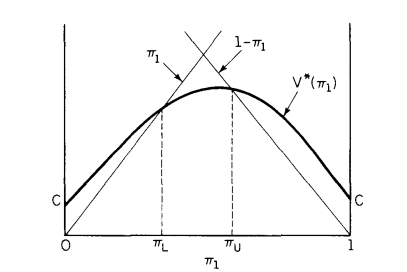
\includegraphics[scale=0.8]{Figures/bayesseqrule.png}
\caption{Relationships yielding the Bayes sequential rule for uniform costs of errors and cost C per sample.}
\label{fig:fig1}
\end{figure}
The function $V^*(\pi_1)$ is a concave (because it is minimum of linear functions), continuous function of $\pi_1$ and $V^*(0)=V^*(1)=C$. Fig. \ref{fig:fig1} also shows the variation of Bayes risk with $\pi_1$ for two other sequential rules: one which decides $H_1$ without taking any samples ($\phi_0=1=\delta_0)$ and the other which decides $H_0$ without taking any samples ($\phi_0=1=1-\delta_0)$. The abscissa of the intersection of the latter two plots with the plot of $V^*(\pi_1)$ give $\pi_L$ and $\pi_U$ respectively.
\paragraph{Rules:} It follows that
\begin{enumerate}
\item if $\pi_1\leq\pi_L$, then the optimum sequential rule is $\phi_0=1=1-\delta_0$
\item if $\pi_1\geq\pi_U$, then the optimum sequential rule is $\phi_0=1=\delta_0$
\item if $\pi_L<\pi_1<\pi_U$, then the optimum sequential rule consumes $N\geq1$ samples.
\end{enumerate}
After taking one sample $y_1$, it is as if our prior on $\{H_0,H_1\}$ has changed to a posterior distribution
$\pi_1(y_1)=\mathbb{P}[H_1\ is\ true\ | Y_1=y_1]$. Therefore, we can recursively apply the original rules (The shape of $V^*$ is not affected by having the knowledge of $Y_1$ as the samples are independent.
\par \emph{Optimum Bayesian sequential decision rule:} The test continues sampling until $\pi_1(y_1,\cdots,y_n)=\mathbb{P}[H_1\ \te{is\ true}|Y_1=y_1,\dots,Y_n=y_n]$ goes out of the interval $(\pi_L,\pi_U)$ and chooses $H_0$ or $H_1$ based on the value of $\pi_1(y_1,\dots,y_n)$. The stopping rule and the terminal decision rule are obtained as
\begin{align}
\phi_n(y_1,\cdots,y_n)&= \begin{cases}0, &\text{if}\  \pi_1(y_1,\dots,y_n)\in [\pi_L,\pi_U],\\1, &\text{if}\  \pi_1(y_1,\dots,y_n)\notin [\pi_L,\pi_U],
\end{cases}\\ \te{and}~\delta_n(y_1,\cdots,y_n)&= \begin{cases}1, & \text{if}\  \pi_1(y_1,\cdots,y_n)\geq \pi_U,\\0,  & \text{if}\  \pi_1(y_1,\cdots,y_n)\leq \pi_L,\\arbitrary, &  \text{otherwise,}\end{cases}
\end{align}
where $\pi_1(y_1,\cdots,y_n)=\mathbb{P}[H_1|Y_1=y_1,\cdots,Y_n=y_n]$.\\
\begin{figure}
\centering
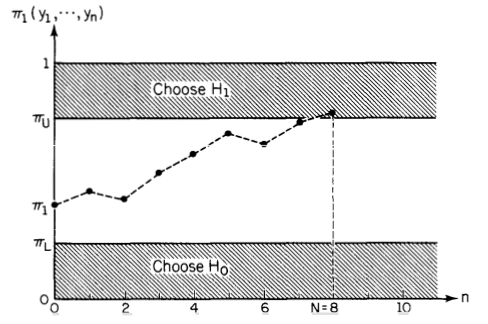
\includegraphics[scale=0.7]{Figures/bayesseqtest.png}\\
\caption{Depiction of realization of a Bayes sequential test}
\end{figure}
The test terminates (under mild conditions) as $\pi_1(y_1,\dots,y_n)$ converges to $1$ under $H_1$ or $0$ under $H_0$ almost surely.
\end{document}